%!TEX root = ../notas_de_clase.tex

\section{Regresión Lineal}

El problema de regresión buscar determinar la relación entre una variable denominada \emph{dependiente} (salida, respuesta o etiqueta) y una variable denominada \emph{independiente} (entrada, estímulo o instancia). Intuitivamente, un modelo de regresión permite entender cómo cambia la variable dependiente cuando la variable independiente es modificada. Esta relación entre ambas variables es representada por una función, consecuentemente, el problema de regresión es equivalente a encontrar una función. De esta forma, en base a (i) el espacio de posible funciones donde se busque dichas relación (por ejemplo el espacio de todos los polinomios de grado menor o igual a 5), y a (ii) el criterio de búsqueda que se aplique, se obtendrán distintos métodos de regresión. 

El modelo básico de regresión, y que sirve de base para modelos más expresivos, es el de regresión lineal. En cuyo caso el espacio de funciones donde se busca la relación entre las variables dependientes e independientes es el de las funciones lineales afines. 

Específicamente, para un conjunto de observaciones de entradas ($x$) y salidas ($y$) de la forma
\begin{equation}
	\{(x_i,y_i)\}_{i=1}^N\subset \R^M \times \R,
	\label{eq:training_set}
\end{equation}
la regresión lineal busca encontrar un modelo lineal, es decir,  
\begin{align}
  f \colon \R^M &\to \R\nonumber\\
  x &\mapsto f(x)=a^\top x + b,\quad a\in\R^M,b\in\R,
 \label{eq:reg_lin_fn} 
\end{align}
que \emph{mejor represente} la forma en que la variable $y$ depende de la variable $x$, esto en base a las las observaciones descritas en la ecuación~\eqref{eq:training_set}.

\vspace{1em}
\noindent\red{\bf Pendiente: ¿por qué lineal? por fácil y por optimalidad bajo supuesto de gaussianidad}


\subsection{Mínimos cuadrados} % (fold)
\label{ssub:min_cuad}
En el contexto recién presentado, aflora naturalmente la siguiente pregunta: \emph{¿cuál es la mejor representación de los datos?} o, equivalentemente, \emph{¿cómo cuantificar la bondad de un modelo de regresión lineal?} Una práctica ampliamente utilizada es elegir la función $f(\cdot)$ en la eq.~\eqref{eq:reg_lin_fn} siguiendo el criterio de \textbf{mínimos cuadrados}. Es decir, elegir la función $f(\cdot)$ que minimiza la suma del cuadrado de las diferencias entre las observaciones y las predicciones calculadas por la función es mínima denotada por el costo
\begin{equation}
	J = \frac{1}{2}\sum_{i=1}^N(y_i-f(x_i))^2.
	\label{eq:least_squares_cost}
\end{equation}
Es decir, la (o las) funciones que satisfacen el criterio de mínimos cuadrados están dadas por\footnote{La constante $\frac{1}{2}$ que multiplica al costo cuadrático no afecta la solución y está ahí por simplicidad de notación cuando se calculen las derivadas de esta expresión.} 
\begin{equation}
	f^\star = \argmin_{f} J.
\end{equation}
En el caso lineal, resolver este problema de optimización es equivalente a encontrar los parámetros $a$ y $b$ en la ec.~\eqref{eq:reg_lin_fn}. Es decir: 
\begin{equation}
	a^\star,b^\star = \argmin_{a,b} \frac{1}{2}\sum_{i=1}^N(y_i-a^
	\top x_i + b)^2
	\label{eq:lin_least_squares}
\end{equation}

Observe que la ecuación anterior es cuadrática en $a$ y $b$, por lo cual tiene un único mínimo que puede ser encontrado explícitamente. Para esto, como la función $f$ en la ecuación~\eqref{eq:reg_lin_fn} no es lineal sino que \emph{afín}, hacemos el siguiente cambio de variable:
\begin{equation}
  \left[ \begin{matrix}x \\  1\end{matrix}\right] \mapsto \tx\in\R^{M+1},\quad
  \left[ \begin{matrix}a \\  b\end{matrix}\right]\mapsto \theta\in\R^{M+1},
 \label{eq:truco_reg_lin} 
\end{equation}
con lo cual el funcional cuadrático a minimizar se convierte en
\begin{equation}
	J = \frac{1}{2}\sum_{i=1}^N(y_i-\theta^
	\top \tx_i)^2
	\label{eq:lin_least_squares2}
\end{equation} 
y el parámetro $\theta$ de mínimos cuadrados puede ser encontrado aplicando las condiciones de primer orden de la siguiente forma:
\begin{align}
\nabla_\theta J=0 &\Leftrightarrow \sum_{i=1}^N(y_i-\theta^\top \tx_i)\tx_i^\top=0  							&&\text{def. $J$}\nonumber\\  
&\Leftrightarrow \sum_{i=1}^Ny_i\tx_i^\top = \sum_{i=1}^N\theta^\top \tx_i\tx_i^\top					&&\text{ordenar}\nonumber\\
&\Leftrightarrow \theta^\top = \sum_{i=1}^Ny_i\tx_i^\top \left(\sum_{i=1}^N \tx_i\tx_i^\top\right)^{-1}	&&\text{despejar $\theta^\top$}\nonumber\\
&\Leftrightarrow \theta =  \left(\sum_{i=1}^N \tx_i\tx_i^\top\right)^{-1} \sum_{i=1}^N \tx_i y_i 		&&\text{transponer}\nonumber\\
&\Leftrightarrow \theta = \left(\tX^\top\tX \right)^{-1} \tX^\top Y 											&&\text{def. $\tX$ y $Y$} \label{eq:sol_mse}
\end{align}
donde $\tX$ y $Y$ son las matrices de datos definidas por




\begin{equation}
  \tX = \left[ \begin{matrix}\tx_1^\top \\\vdots \\ \tx_N^\top \end{matrix}\right]\in\R^{N\times (M+1)} ,\quad
  Y = \left[ \begin{matrix}y_1 \\\vdots \\y_N \end{matrix}\right] \in\R^{N}
 \label{eq:matrices_X} 
\end{equation}

La Figura \ref{fig:reg_lin_1} muestra un ejemplo de regresión lineal para observaciones de chirridos por segundo en función de la temperatura. 

\begin{figure}[H]
	\centering
	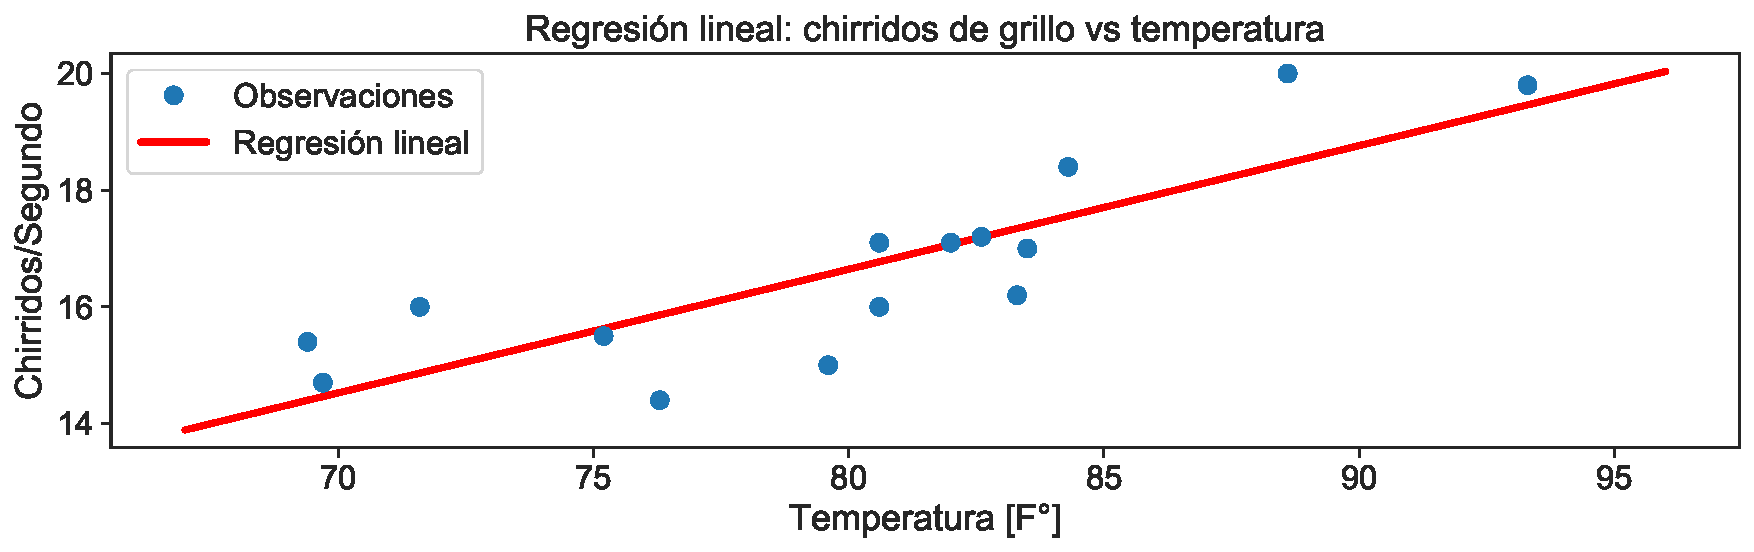
\includegraphics[width=0.9\textwidth]{img/cap1_chirridos.pdf}\\
	\caption{Ejemplo de regresión lineal.}
	\label{fig:reg_lin_1}
\end{figure}

La expresión $\left(\tX^\top\tX \right)^{-1} \tX^\top$ en la ecuación~\eqref{eq:sol_mse} es conocida como la pseudo-inversa de Moore-Penrose \cite[p.~7]{benisrael_greville_2006}. Observe que una condición necesaria para que esta pseudo-inversa esté bien definida es que la cantidad de observaciones ($N$) sea mayor o igual que las dimensiones ($M+1$). Esto es porque la matriz $\tX^\top\tX$ es de tamaño $(M+1)\times(M+1)$ y su rango es $\min \{N, M+1\}$, consecuentente, para que $\tX^\top\tX$ tenga rango completo (y por ende sea invertible) se debe cumplir al menos que $N\geq M+1$. Para encontrar una condición necesaria y suficiente para la existencia de la solución de mínimos cuadrados en la ecuación \eqref{eq:sol_mse}, además de el número de observaciones $N\geq M+1$ se requiere que éstas no sean colineales, pues de esta forma los términos que componen la pseudo-inversa son efectivamente linealmente independiente y ésta tiene rango completo. 

En la práctica, es usual que tengamos más observaciones que parámetros, cuando consideramos un modelo lineal (o lineal generalizado, como veremos a continuación). Sin embargo, es posible que las observaciones sean \emph{redundantes}, es decir, no exactamente iguales (y por ende linealmente independientes) pero suficientemente parecidas para que la inversa de Moore-Penrose esté \emph{cercana} a ser no invertible. Esto puede resultar en problemas de inestabilidad numérica al  calcular la inversa de $\tX^\top\tX$. Una forma de evitar este problema penalizar soluciones que son \emph{cercanas a ser no invertibles} o \emph{irregulares}, de forma similar que se penalizan funciones que no representan bien los datos, en el sentido del error cuadrático. Este procedimiento se refiere a \emph{regularizar} la solución.

\vspace{1em}
\noindent\red{\bf Pendiente: Discutir interpretación geométrica del criterio de mínimos cuadrados  con la siguiente figura}

\begin{figure}[ht]
	\centering
	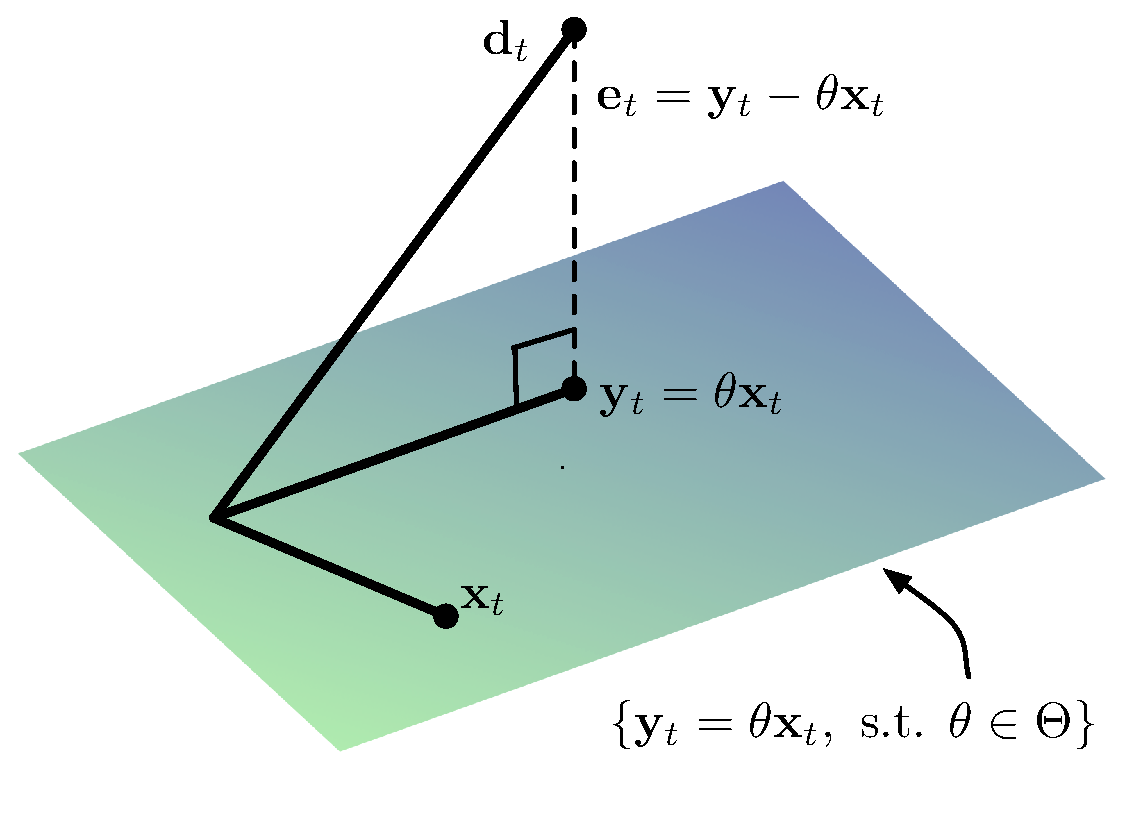
\includegraphics[width=0.5\textwidth]{img/projection.pdf}\\
	\caption{Interpretación geométrica de la regresión lineal y mínimos cuadrados}
	\label{fig:projection}
\end{figure}

% subsubsection Mínimos cuadrados (end)

\subsubsection{Mínimos cuadrados regularizados} % (fold)
\label{ssub:min_cuad_reg}

El criterio para encontrar los parámetros del modelo de regresión lineal puede, además de considerar el ajuste de la función a las observaciones, incluir ciertas penalizaciones sobre los modelos o soluciones a elegir. Estas penalizaciones pueden ser codificadas directamente en la función de costo, consecuentemente, ésta tiene ahora consta de un término que penaliza el ajuste de los datos y otro término que penaliza soluciones que se alejan de lo deseado. Un criterio estándar de penalización es la norma de los parámetros, es decir, 
\begin{equation}
	J_\rho = \frac{1}{2}\sum_{i=1}^N(y_i-\theta^
	\top \tx_i)^2 + \frac{\rho}{p}||\theta||_p^p,\ p\in\R_+,
	\label{eq:reg_least_squares}
\end{equation} 
donde $||\cdot||_p$ denota la norma $\ell_p$, es decir, $||\theta||_p=\left(\sum_{j=1}^N|\theta_j|^p\right)^\frac{1}{p}$ y el parámetro $\rho$ tiene el rol de balancear la importancia entre ajuste (primer término) y regularidad de la solución (segundo término). Distintos valores de $p$ inducen distintos propiedades sobre las soluciones, siendo las más usadas las correspondientes a $p=1$ denotado por \textbf{Lasso} \cite{tibshirani_1996} o bien $p=2$ denotado por regularización de \textbf{Tikhonov} \cite{tikhonov_arsenin_1977} o bien \textbf{\emph{Ridge Regression}} \cite{hoerl_kennard_1970}.  

Una ventaja de la regularización de Tikhonov es que su solución, al igual que el caso de mínimos cuadrados no regularizados, puede ser encontrada en forma exacta. En efecto, como para $p=2$ tenemos que el término de regularización puede ser expresado como $||\theta||_2 = \theta^\top\theta$, con lo que el minimizante del costo cuadrático regularizado está dado por: 
\begin{align}
\nabla_\theta J_\rho=0 &\Leftrightarrow \sum_{i=1}^N(\theta^\top \tx_i - y_i)\tx_i^\top + \rho\theta^\top=0  							&&\text{def. $J$}\\  
&\Leftrightarrow \sum_{i=1}^Ny_i\tx_i^\top = \sum_{i=1}^N\theta^\top \tx_i\tx_i^\top + \rho\theta^\top					&&\text{ordenar}\\
&\Leftrightarrow \theta^\top = \sum_{i=1}^Ny_i\tx_i^\top \left(\sum_{i=1}^N \tx_i\tx_i^\top + \rho \eye\right)^{-1}	&&\text{despejar $\theta^\top$}\\
&\Leftrightarrow \theta =  \left(\sum_{i=1}^N \tx_i\tx_i^\top +\rho \eye\right)^{-1} \sum_{i=1}^N \tx_i y_i 		&&\text{transponer}\\
&\Leftrightarrow \theta = \left(\tX^\top\tX +\rho \eye\right)^{-1} \tX^\top Y 											&&\text{def. $\tX$ y $Y$}
\end{align}

De la última expresión, es posible ver que el requerimiento de que las observaciones disponibles sean (i) más que la dimensión $M+1$ y que además (ii) éstas sean colineales ya no es necesario para que la solución esté bien definida. De hecho, la matriz $\tX^\top\tX$ puede efectivamente estar cercana a ser no invertible, sin embargo, es posible \emph{regularizar} la solución forzando que la matriz $\left(\tX^\top\tX +\rho \eye\right)$ sea efectivamente \emph{regular} aumentando el valor de $\rho$. 

En el caso de la regularización de Tikhonov, se entiende por soluciones regulares las que están definidas por parámetros que tienen una norma pequeña, tal como lo sugiere la ecuación \eqref{eq:reg_least_squares}. Sin embargo, es posible aplicar otros criterios de regularidad, por ejemplo, una solución regular puede ser una en la cual la mayoría de los de parámetros son idénticamente nulos, esto es conocido como una solución \textbf{rala} o \textbf{\emph{sparse}}. Usando por costo de regularización el número de parámetros no nulos (definido por la ``norma'' $l_0$) en la definición del costo en la ecuación \eqref{eq:reg_least_squares}, es posible determinar cuáles son las soluciones que utilizan menos variables independientes para representar la variable dependiente. Desafortunadamente, resolver encontrar la solución usando la ``norma'' $l_0$ es muy difícil, sin embargo, bajo ciertas condiciones la consideración de la norma $l_1$ puede llevar a la misma solución.

\vspace{1em}
\noindent\red{\bf Referencias pendiente: Compressed sensing, sparse feature selection}



\subsubsection{Máxima verosimilitud} % (fold)
\label{ssub:max_ver}

Ahora tomaremos un enfoque distinto, en el cual no buscaremos el modelo que menor discrepancia tiene con los datos, sino que vamos a elegir el modelo que \emph{más probablemente} haya generado los datos. La diferencia fundamental en este caso es que necesitamos diseñar un modelo que generó exactamente los datos, lo cual requiere modelar el ruido de las observaciones. 

Consideremos el siguiente modelo
\begin{equation}
	y = \theta^\top\tx + \epsilon,\quad \epsilon\sim\cN(0,\sigma_\epsilon^2) \ \text{i.i.d.} 
	\label{eq:lin_gauss}
\end{equation}
el cual representa la variable dependiente $y$ mediante una parte determinística que depende linealmente de $\tx$ y una parte aleatoria. El modelo probabilístico en la ecuación~\eqref{eq:lin_gauss} puede expresarse en forma distribucional como 
\begin{equation}
	y|\tx \sim p(y|\tx,\theta) = \cN(y;\theta^\top\tx,\sigma_\epsilon^2).
\end{equation}
Adicionalmente, como las observaciones son \emph{condicionalmente independiente dado el modelo}, la probabilidad de todo el conjunto de entrenamiento $T=\{(x_i,y_i)\}_{i=1}^N$ es factorizable y dada por
\begin{equation}
	p(Y|\tX,\theta) = p(y_1,\ldots,y_N|\tx_1,\ldots,\tx_N,\theta)= \prod_{i=1}^Np(y_i|\tx_i,\theta) = \prod_{i=1}^N \cN(y_i;\theta^\top\tx_i,\sigma_\epsilon^2).
\end{equation}

El ajuste del modelo entonces puede hacerse mediante la maximización (con respecto a $\theta$) de la probabilidad que dicho modelo haya generado los datos de entrenamiento en la ecuación~\eqref{eq:training_set}. Es decir: 

\begin{equation}
	\theta^\star = \argmax p(y_1,\ldots,y_N|\tx_1,\ldots,\tx_N,\theta)
\end{equation}
en el caso de arriba, las observaciones son condicionalmente independientes, y su distribución está dada por la ecuación~\eqref{eq:lin_gauss}. Consecuentemente:

\begin{align}
	\theta^\star 	&= \argmax \prod_{i=1}^Np(y_i|\tx_i,\theta)\\
					&= \argmax \prod_{i=1}^N \cN(y_i;\theta^\top\tx_i,\sigma_\epsilon^2) \\
					&= \argmax \prod_{i=1}^N \frac{1}{\sqrt{2\pi}\sigma_\epsilon} \exp\left({\frac{-1}{2\sigma_\epsilon^2}(y_i-\theta^\top\tx_i)^2}\right) \\
					&= \argmin \sum_{i=1}^N (y_i-\theta^\top\tx_i)^2
\end{align}
La misma solución exacta que mínimos cuadrados, la diferencia es que también podemos maximizar con respecto a la varianza del ruido.

% subsubsection máxima_verosimilitud (end)

\centerline{--------------------------------- clase 27/3/18 ---------------------------------}

\subsubsection{Regresión Bayesiana} % (fold)
\label{ssub:map}
\noindent\textbf{Repaso probabilidades - pending}\\

\noindent\textbf{Tres pasos de inferencia Bayesiana}
\begin{itemize}
	\item Definir un modelo conjunto para todas las cantidades involucradas, observaciones, valores futuros, parametros, etc
	\item Ajustar el modelo a la luz de observaciones
	\item Evaluar el modelo e interpretar resultados
\end{itemize}




En vez de maximizar la probabilidad de que los datos hayan sido generado por el modelo propuesto, podemos calcular la distribución condicional sobre modelos dado el conjunto de observaciones, es decir, $p(\theta|T)$. Esta es conocida como \emph{distribución posterior del modelo dado los datos} y mediante el teorema de Bayes puede expresarse como

\begin{equation}
	p(\theta|T)=\frac{p(Y|\theta,\tX)p(\theta,\tX)}{p(Y|\tX)}
	\label{eq:posterior}
\end{equation}

\noindent\textbf{Observaciones:}\\

\noindent 1) La constante de normalización es en general muy complicada de calcular, pues es la probabilidad de que la salida sea $Y$ para una entrada $\tx$ y \emph{cualquier} modelo, de hecho, 

\begin{equation}
		p(Y|\tX) 	= 	\int p(Y,\theta|\tX)\td \theta 
					= 	\int p(Y|\theta,\tX) p(\theta) \td \theta
\end{equation}

Sin embargo, nótese que $p(Y|\tX)$ es solo una constante de normalización y como $p(\theta|T)$ es una función de $\theta$, el denominador en ecuación~\eqref{eq:posterior} solo amplifica dicha función. Es decir 

\begin{equation}
	p(\theta|T)\propto p(Y|\theta,\tX)p(\theta,\tX)
	\label{eq:posterior2}
\end{equation}

La distribución posterior es entonces una \emph{mezcla} entre la distribución posterior (que representa la creencia en la variable antes de ver datos) y la verosimilitud (que representa la probabilidad de los datos condicional al modelo). Cuando la distribución a priori y a posteriori son de la misma familia, diremos que son distribuciones conjugadas y además que el prior es un \emph{prior} conjugado para la verosimilitud. Ejemplos de priors conjugados son las distribuciones gaussianas, por ejemplo, si consideramos $p(\theta,\tX) = \cN(0,\sigma_\theta^2)$ y una verosimilitud gaussiana (i.e., modelo linear con ruido gaussiano), tenemos

\begin{align}
	p(\theta|T)	&\propto p(Y|\theta,\tX)p(\theta,\tX)\\
				&= \cN(Y;\theta^\top\tX,\eye\sigma_\epsilon^2)\cN(\theta;0,\sigma_\theta^2)\\
				&=\cN(\theta; \mu,\Sigma)
\end{align}

\noindent\textbf{Observaciones:}\\
\noindent 1) ¿y la constante de normalización?

\doublebox{
\begin{minipage}{\linewidth}
\textbf{\underline{Ejemplo:}}

Otro caso de priors conjugados es la distribución binomial, que consiste en la probabilidad de obtener $s$ aciertos en $n$ intentos, cada uno independientes y equiprobables con probabilidad desconocida $q$.

\begin{equation}
	p(n, s) = \binom{n}{s} q^s (1-q)^{n-s}
\end{equation}

Donde su prior conjugado es la distribución Beta con parámetros ($\alpha, \beta$)

\begin{equation}
	p(q) = \frac{q^{\alpha-1}(1-q)^{\beta-1}}{\mathcal{B}(\alpha, \beta)}
\end{equation}

Donde $\mathcal{B}(x,y)$ es la función Beta que actua como factor normalizador.


Luego, si queremos obtener la posterior de $q$ con un prior Beta,

\begin{align}
	p(q|n,s) & = \frac{p(n.s|q)p(q)}{p(n,s)} \\
			 & = \frac{\binom{n}{s}q^s(1-q)^{n-s}q^{\alpha-1}(1-q)^{\beta-1}}{p(n,s)} \\
			 & = \textcolor{blue}{
			 \underbrace{\frac{\binom{n}{s}}{p(n,s)}
			 }}
			 q^s(1-q)^{n-s}q^{\alpha-1}(1-q)^{\beta-1}\\
			 & = \textcolor{blue}{\mathcal{B}(s+\alpha, \beta + n - s)} q^{s + \alpha-1} (1-q)^{n-s+\beta-1} && \text{Es una distribución Beta}
\end{align}
\textbf{\underline{Aplicación:}}

Se sabe que el $1\%$ de las mujeres tienen cancer de mamas, y se tienen un test para detectar si una mujer lo presenta o no. Si la paciente tiene cancer (C), el test dará postitivo (PT) con una probabilidad del $80\%$ y negativo (NT) con $20\%$, en cambio cuando la paciente está sana (NC), hay un $9.6\%$ de probabilidad que el test salga erroneo y si detecte cancer.

Una paciente se realiza el test y este sale positivo, nos gustaría obtener la probabilidad de que en realidad tenga cancer dado este resultado.

\begin{align}
	p(C|PT) & =\frac{p(PT|C)p(C)}{p(PT)} \\
			& = \frac{p(PT|C)p(C)}{p(PT|C)p(C)+p(PT|NC)p(NC)} \\
			& = \frac{0.8 \cdot 0.001}{0.8 \cdot 0.01 + 0.096 \cdot 0.99}\\
			& = 0.0776
\end{align}

De esta misma forma podemos completar todos los casos.
\\
% \begin{table}%[H]
\centering
\begin{tabular}{c|cc}
\toprule
   & C ($1\%$) &  NC($99\%$) \\\hline
PT & $0.8$ & $0.096$\\
NT & $0.2$ & $0.904$ \\
\bottomrule
\end{tabular}
\captionof{figure}{Resumen de las probabilidades para el caso del test de cancer.}
\label{table:cancer}
% \end{table}

\end{minipage}}


% subsubsection máximo_a_posteriori (end)

\subsection{Maximo a posteriori} % (fold)
\label{sub:map}

¿Cuál es el equivalente a regularizar en es sentido probabilístico? La respuesta está en asignar más probabilidad \emph{a priori} antes de ver datos en vez de penalizar y encontrar (una) moda de la distribución posterior, es decir 


\begin{align}
	\theta_\text{MAP}^\star 	&= \argmax p(Y|\theta,\tX)p(\theta,\tX)\\
								&= \argmax \prod_{i=1}^Np(y_i|\tx_i,\theta)p(\theta,\tX)\\
								&= \argmax \prod_{i=1}^N \cN(y_i;\theta^\top\tx_i,\sigma_\epsilon^2)\cN(\theta;0,\sigma_\theta^2) \\
								&= \argmax \prod_{i=1}^N \frac{1}{\sqrt{2\pi}\sigma_\epsilon} \exp\left({\frac{-1}{2\sigma_\epsilon^2}(y_i-\theta^\top\tx_i)^2}\right)
											\frac{1}{(\sqrt{2\pi}\sigma_\theta)^{M+1}} \exp\left({\frac{-||\theta||^2}{2\sigma_\theta^2}}\right) \\
								&= \argmax  \frac{1}{\sqrt{2\pi}\sigma_\epsilon} \frac{1}{(\sqrt{2\pi}\sigma_\theta)^{M+1}}
											\exp\left( \sum_{i=1}^N{\frac{-1}{2\sigma_\epsilon^2}(y_i-\theta^\top\tx_i)^2} -{\frac{||\theta||^2}{2\sigma_\theta^2}}\right) \\
								&= \argmin \sum_{i=1}^N{(y_i-\theta^\top\tx_i)^2} +{\frac{\sigma_\epsilon^2}{\sigma_\theta^2}||\theta||^2}\quad {\tt (:|)}
\end{align}

\subsection{Predicciones} % (fold)
\label{sub:predicciones}
Una vez que el modelo está ajustado, ya sea con estimaciones paramétricas puntiales o distribucionales, ¿cómo hacemos predicciones? En el caso puntual, la predicción es simplemente evaluar el modelo en el parámetro encontrado $\theta$ y la entrada $x$. En el caso de la estimación bayesiana del parámetro, la predicción toma en cuenta todos los posibles valores del parámetro. En efecto, la distribución de la variable dependiente $y$ para una nueva entrada $x$ está dada por la distribución condicional del $y$ dado todos los datos de entrenamiento, es decir, 

\begin{equation}
 	p(y|x,\{(x_i,y_i)\}_{i=1}^N) = \int p(y|x, \theta)p(\theta|\{(x_i,y_i)\}_{i=1}^N) d\theta
 \end{equation} 

consecuentemente, la esperanza está dada por

\begin{align}
	\E{y|x,\{(x_i,y_i)\}_{i=1}^N} 
	&= \int y p(y|x,\{(x_i,y_i)\}_{i=1}^N) dy\\
	&= \int y p(y|x, \theta)p(\theta|\{(x_i,y_i)\}_{i=1}^N) d\theta dy\\
	&= \int y \cN(y;\theta^\top xp,\sigma_e^2)\cN(\theta;\mu_\theta, \sigma_\theta^2) d\theta dy\\
	&= \int \theta^\top x\cN(\theta;\mu_\theta, \sigma_\theta^2) d\theta \\
	&= \mu_\theta^\top x
\end{align}

% subsection predicciones (end)

\subsection{Inference beyond supervised learning} % (fold)
\label{sub:inference_beyond_supervised_learning}

% subsection inference_beyond_supervised_learning (end)
